\subsection{Verification of the Velocity Model}
In the former section a approximation of the velocity model has been established. 


\begin{figure}[H]
  \centering
 	%Trim margins @:   left        bottom       right       top
 	\adjustbox{ trim = {.15\width} {.30\height} {.15\width} {.30\height}, clip }
  {
    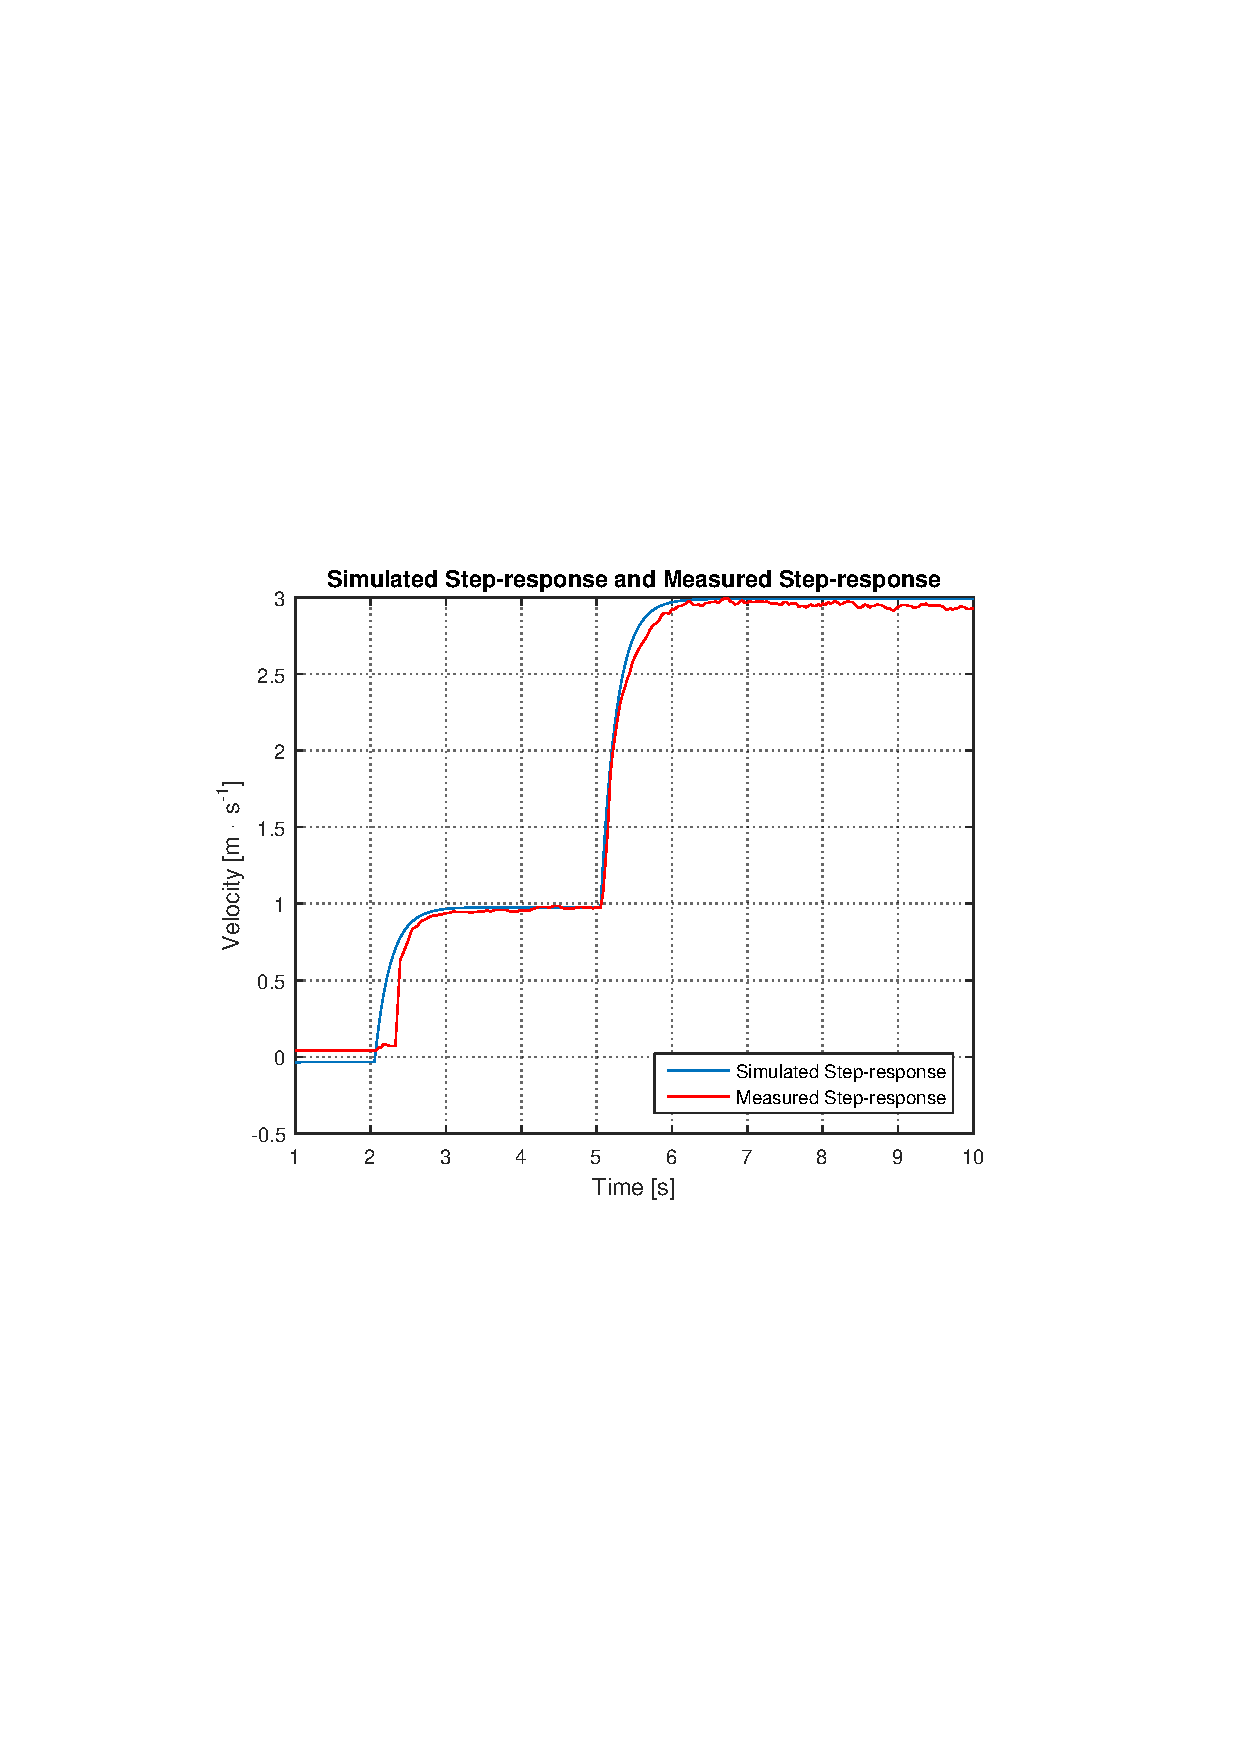
\includegraphics[width=1.2\textwidth]{figures/SimulationIRLsteprespons2.pdf}
  }
  \caption{A plot of a measured armature resistance, with a red line indicating the an average value.}
  \label{armatureResistance}
\end{figure}



Hvad sker der i testen?

Hvordan ser det ud når jeg sammenligner dem

Rød pup i starten er sensor lag

Det er en approximation


\begin{itemize}
\item Uneven belts 
\item Uneven floor
\item Belts slipping on the floor
\item Wear and tear on the internal gears
\end{itemize}